\section{实验结果及分析}
\subsection{仿真图}
\begin{figure}[htbp]
    \centering
    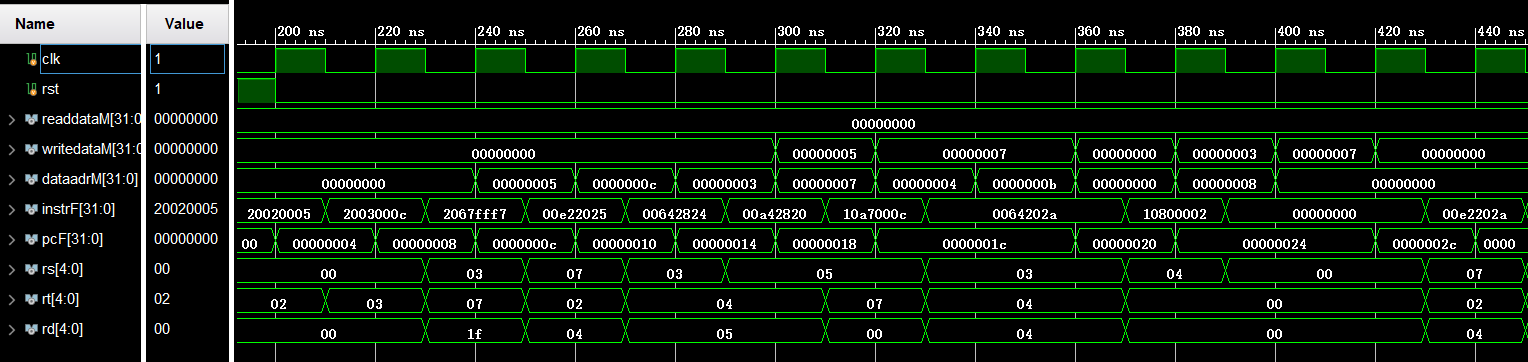
\includegraphics[width=0.9\textwidth]{r1.png}
    \label{fig:my_label}
\end{figure}
\begin{figure}[htbp]
    \centering
    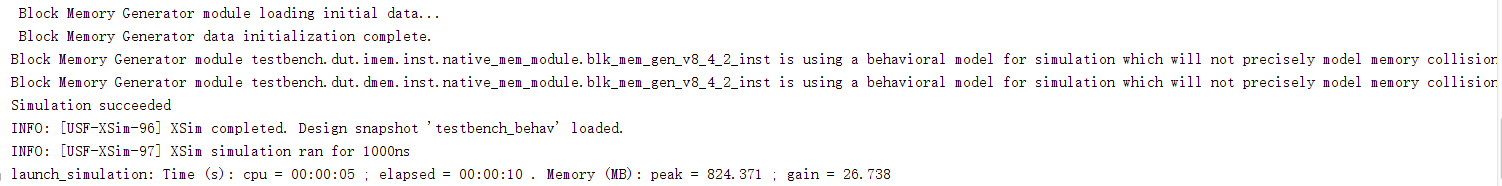
\includegraphics[width=0.9\textwidth]{r2.png}
    \label{fig:my_label}
\end{figure}

\subsection{控制台输出}
\begin{figure}[htbp]
    \centering
    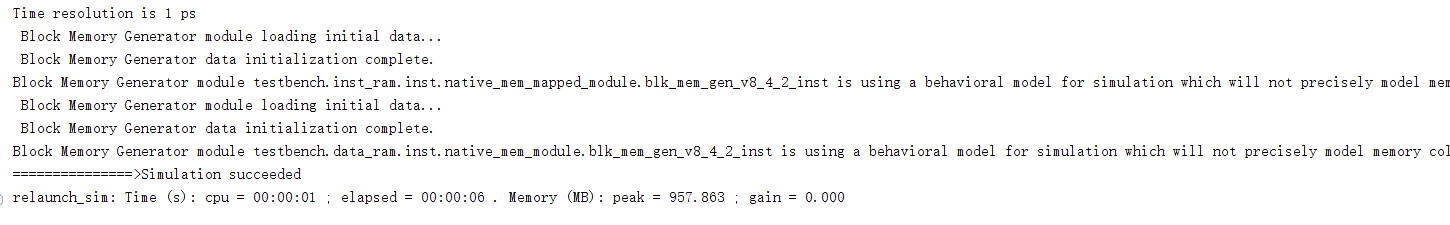
\includegraphics[width=0.9\textwidth]{r3.png}
    \label{fig:my_label}
\end{figure}

\subsection{结果分析}
\begin{enumerate}
    \item R型数据冒险:指令为00e22025时,$4 = $7 or $2,其下一条指令为00642824,$5 = $3 and $4,会用到上一条指令的四号寄存器,但由于写回是在第五阶段发生,所以在alu计算完后,就应该将结果前推到下一条指令的execute阶段。
    所以如果当前使用的rsE地址与writeregM相等,则将memory阶段的aluoutM前推;如果与writereW相等,则将writeback阶段的resultW前推。当前情况是将上一条指令的aluoutM前推。
    \item lw数据冒险:指令为8c020050时,$2 = [80],后面第二条指令为ac020054,需要用到$2。首先判断decode 阶段 rs 或 rt 的地址是否是 lw 指令要写入的地址,若相等则使stallD和stallF信号有效。
    并且使E阶段寄存器刷新。
    \item beq控制冒险:指令为10800001是,beq指令发生,但发生时,该指令的后三条指令已经进入流水线,这时需要将这三条指令产生的影响全部清除。
    将分支指令的判断提前至 decode 阶段,此时能够减少两条指令的执行,只需再刷新他的后一条指令即可。在 regfile 输出后添加一个判断相等的模块,并解决新出现的数据冒险,即可提前判断 beq
\end{enumerate}